\documentclass[lettersize,journal]{IEEEtran}
\usepackage{amsmath,amsfonts}
\usepackage{algorithmic}
\usepackage{algorithm}
\usepackage{array}
\usepackage[caption=false,font=normalsize,labelfont=sf,textfont=sf]{subfig}
\usepackage{textcomp}
\usepackage{stfloats}
\usepackage{url}
\usepackage{verbatim}
\usepackage{graphicx}
\usepackage{cite}
\hyphenation{op-tical net-works semi-conduc-tor IEEE-Xplore}
% updated with editorial comments 8/9/2021

% Marker for details only the authors can supply. Search for "TODO" before submission.
\newcommand{\todo}[1]{\textbf{[TODO: #1]}}

\begin{document}

\title{Reproducing DFF-Adapter: Fine-Grained DINOv2 Tuning with Dual Supervision for Face Forgery Detection and Its Cross-Dataset Generalization}

\author{Author1-RollNo., Author2-RollNo. \todo{names and roll numbers from the SOP}}

\maketitle

\begin{abstract}
Deepfake detectors that score highly on their training benchmark often fail on unseen manipulations. We re-implement DFF-Adapter~\cite{zhang2026dff}, a parameter-efficient detector that inserts multi-head LoRA-expert adapters, with a shared head and task-specific heads, into the query, value and output projections of every transformer block of a frozen DINOv2 backbone, and trains authenticity detection jointly with forgery-type classification. Because of compute limits we use DINOv2-Small and DINOv2-Base instead of the paper's DINOv2-Large. Trained on FaceForensics++ (c23), our best configuration (Small, 30 epochs) reaches 99.08\% FF++ validation video AUC (paper: 99.56\%, test split) and 82.98\%, 86.25\% and 88.03\% video AUC on Celeb-DF-v1, Celeb-DF-v2 and a 392-video DFDC subset (paper: 96.14\%, 95.26\% and 89.96\%). The gap to the paper is therefore 9--13 percentage points (pp) on Celeb-DF but under 2~pp on our DFDC subset, whose composition may differ from the paper's. A larger backbone did not improve our cross-dataset results: Base trails Small by 4.03~pp video AUC on DFDC. As an extension, label smoothing (0.1) on the forgery-type loss did not improve video-level AUC on any unseen set. All results are single-seed and use different checkpoints for different datasets; see Section~\ref{sec:lim}.
\end{abstract}

\begin{IEEEkeywords}
Deepfake detection, DINOv2, LoRA, mixture of experts, parameter-efficient fine-tuning, cross-dataset generalization, label smoothing.
\end{IEEEkeywords}

\section{Introduction}
Synthetic face manipulation has become cheap and convincing enough to threaten information integrity, and detection is now a standard stress test for the generalization ability of deep models~\cite{lecun2015deep}. The core difficulty is not accuracy on a known benchmark, which modern detectors saturate, but robustness when the manipulation method, compression, or identity distribution changes.

Recent work therefore adapts large pre-trained vision models. DFF-Adapter~\cite{zhang2026dff} observes that existing DINOv2-based detectors treat the task as generic real/fake classification and typically insert an adapter only into the last block or fine-tune only the last layers. It instead injects low-rank adapters into \emph{every} transformer block and adds an auxiliary forgery-type classification task, so that the authenticity decision can inherit manipulation-specific cues. With 3.5M trainable parameters it reports accuracy comparable to or better than much heavier detectors.

\textbf{Project criterion.} We follow the ``reproduce paper results'' criterion: we re-implemented the method from the paper's description and did not run the authors' implementation, so the paper's numbers below are reference values taken from its publication. \todo{confirm the criterion and whether the authors' code is public}

\textbf{Contributions.}
\begin{itemize}
\item A re-implementation of DFF-Adapter whose trainable-parameter count follows the paper's budget (Section~\ref{sec:method}), evaluated on frozen DINOv2-Small and DINOv2-Base.
\item Evaluation on FF++, Celeb-DF-v1, Celeb-DF-v2 and a DFDC subset, compared side by side with the paper's reported video AUC and EER.
\item Controlled comparisons of backbone size and training length, and one extension: label smoothing on the forgery-type loss.
\item An explicit list of protocol and checkpoint differences that limit what can be concluded.
\end{itemize}

\textbf{Team composition.}
\begin{itemize}
\item Member 1: \todo{name, roll no., e-mail, contribution}
\item Member 2: \todo{name, roll no., e-mail, contribution}
\end{itemize}

\section{Related Work}
\textbf{Classical forgery detectors.} Early detectors target visible or physical artifacts and later learned blending boundaries and synthetic-forgery cues, e.g., Face X-ray~\cite{li2020facexray} and self-blended images~\cite{shiohara2022sbi}, to improve generalization to unseen manipulations. Quality is measured on benchmarks such as FaceForensics++~\cite{rossler2019faceforensics}, Celeb-DF~\cite{li2020celebdf} and DFDC~\cite{dolhansky2020dfdc}.

\textbf{Pre-trained large models.} Vision transformers~\cite{vaswani2017attention,dosovitskiy2021vit} pre-trained at scale provide semantically rich features. DINOv2~\cite{oquab2024dinov2} is a self-supervised backbone with strong transfer; the DFF-Adapter paper uses its registers variant~\cite{darcet2024registers} at Large size, whereas we use the plain Small and Base checkpoints.

\textbf{Parameter-efficient tuning.} LoRA~\cite{hu2022lora} learns low-rank updates to frozen weights and keeps the number of trainable parameters small while preserving pre-training priors.

\textbf{DFF-Adapter.} DFF-Adapter~\cite{zhang2026dff} combines these ideas: low-rank adapters in every transformer block, a Forgery-Aware Multi-Head Router (FAMHR) that splits the channels into heads and routes each head to its top-3 LoRA experts, and Shared-Enhanced Task Fusion (SETF), which fuses a shared head with task-specific heads so that forgery-type knowledge reaches the authenticity stream. The authors report the best overall results across five deepfake benchmarks.

\textbf{Label smoothing.} Label smoothing~\cite{szegedy2016rethinking} softens one-hot targets and is often reported to improve calibration and generalization~\cite{muller2019labelsmoothing}. The paper uses hard forgery-type labels; testing smoothed type labels is our extension.

\section{Proposed Methodology}\label{sec:method}
\subsection{Overview}
Fig.~\ref{fig:pipeline} summarises the model. A $224\times224$ face crop is split into $14\times14$ patches (256 patches plus [CLS], 257 tokens) and encoded by a frozen DINOv2 backbone with 12 transformer blocks. In every block, three linear layers are wrapped as $y=Wx+\Delta Wx$ with the frozen $W$ and a trainable DFF-Adapter: the query, value and attention-output projections. A linear head on the [CLS] token produces the authenticity logit (task 0) or the five-way forgery-type logits (task 1). Only the adapters and the two linear heads are trained.

\begin{figure*}[!t]
\centering
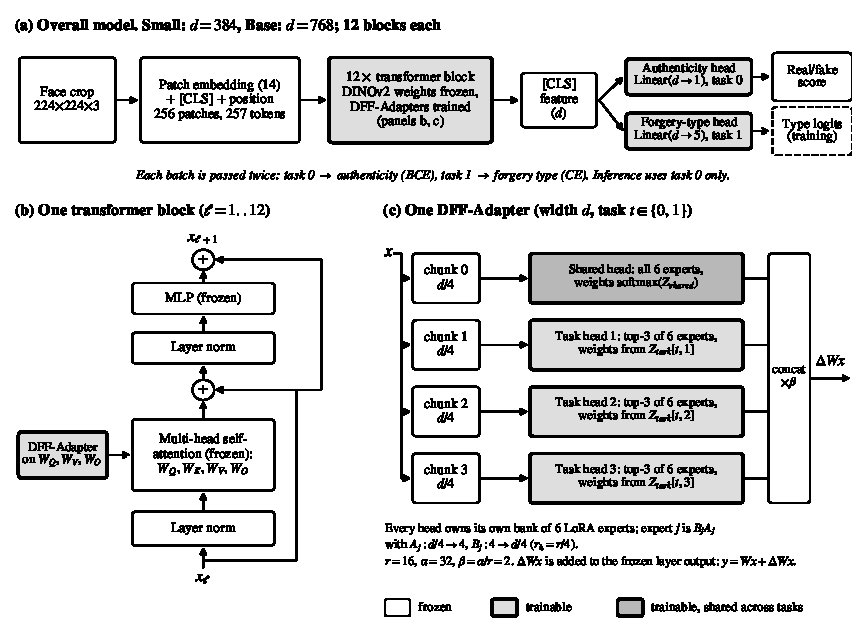
\includegraphics[width=0.86\textwidth]{fig_arch}
\caption{(a) Overall model for both backbones. (b) One transformer block with its adapters. (c) One DFF-Adapter: the input channels are split into four chunks, one handled by the shared head and three by task heads. Shaded components are trained; the DINOv2 weights are frozen. The dashed output is used only in training.}
\label{fig:pipeline}
\end{figure*}

\subsection{DFF-Adapter}
Let $x\in\mathbb{R}^{L\times d}$ be the input of a wrapped layer and $H{=}4$ the number of heads. The channels are split into $H$ chunks $x^{(k)}\in\mathbb{R}^{L\times d/H}$. Each head $k$ owns a bank of $N{=}6$ LoRA experts $(A_j^{(k)},B_j^{(k)})$ with $A_j^{(k)}\in\mathbb{R}^{r_h\times d/H}$, $B_j^{(k)}\in\mathbb{R}^{d/H\times r_h}$ and per-head rank $r_h=r/H=4$, where $r=16$.

\textbf{Task heads} ($k=1,2,3$). For task $t\in\{0,1\}$ (authenticity, forgery type) the routing probabilities are $g_{t,k}=\mathrm{softmax}(Z_{\mathrm{task}}[t,k])$. The top three experts $S_{t,k}$ are kept and their weights renormalised, giving
\begin{equation}
f_t^{k}=\beta\sum_{j\in S_{t,k}}\tilde g_{t,k}^{(j)}\,B_j^{(k)}A_j^{(k)}x^{(k)},\quad
\tilde g_{t,k}^{(j)}=\frac{g_{t,k}^{(j)}}{\sum_{\ell\in S_{t,k}}g_{t,k}^{(\ell)}}.
\label{eq:task}
\end{equation}
\textbf{Shared head} ($k=0$). It mixes all experts with $\mathrm{softmax}(Z_{\mathrm{shared}})$ and is common to both tasks:
\begin{equation}
f_{\mathrm{share}}=\beta\sum_{j=1}^{N}\mathrm{softmax}(Z_{\mathrm{shared}})_j\,B_j^{(0)}A_j^{(0)}x^{(0)}.
\label{eq:shared}
\end{equation}
The head outputs are concatenated along the channel axis, $\Delta Wx=\mathrm{concat}(f_{\mathrm{share}},f_t^{1},f_t^{2},f_t^{3})$, and added to the frozen layer output, with $\beta=\alpha/r=32/16=2$. The routing logits $Z_{\mathrm{task}}\in\mathbb{R}^{2\times3\times6}$ and $Z_{\mathrm{shared}}\in\mathbb{R}^{6}$ are learned parameters per adapter that do not depend on the input; they are initialised from $\mathcal{N}(0,0.5^2)$, a choice of ours. $A$ is initialised uniformly and $B$ at zero, so every adapter starts as the identity. The shared head receives gradients from both losses, which is how forgery-type information reaches the authenticity stream.

\subsection{Backbones and trainable parameters}
We use the frozen \texttt{facebook/dinov2-small} and \texttt{facebook/dinov2-base} checkpoints (no registers); the paper uses \texttt{dinov2-with-registers-large}. One adapter has $H N\cdot 2\,r_h\,(d/H)+2(H{-}1)N+N$ parameters, and there are $3$ adapters per block. Table~\ref{tab:bb} lists the settings and counts. The Small count equals the value logged by our training script; the paper's reported 3.5M is consistent with our formula applied to the Large backbone (about 3.55M).
\begin{table}[!t]
\caption{Backbones (patch size 14, $224\times224$ input) and trainable parameters.\label{tab:bb}}
\centering
\footnotesize
\setlength{\tabcolsep}{3pt}
\begin{tabular}{|l||c|c|c|}
\hline
 & Small & Base & Large\\
\hline
Blocks / hidden size $d$ & 12 / 384 & 12 / 768 & 24 / 1024\\
Native attention heads & 6 & 12 & 16\\
Adapter head width $d/4$ & 96 & 192 & 256\\
Adapter parameters & 665{,}064 & 1{,}328{,}616 & 3{,}541{,}968\\
Two linear heads & 2{,}310 & 4{,}614 & 6{,}150\\
\textbf{Trainable total} & \textbf{667{,}374} & 1{,}333{,}230 & 3{,}548{,}118\\
\hline
\end{tabular}
\end{table}
The Base and Large totals are computed from the closed-form expression, not logged. \todo{confirm the Base total against the ``trainable parameters'' line of a Base run}

\subsection{Dual-supervision objective}
Each batch is passed through the network twice, once per task, and one backward pass is made on
\begin{equation}
\mathcal{L}=\lambda_a\,\mathrm{BCE}\big(s,y_a\big)+\lambda_t\,\mathrm{CE}\big(\mathbf{z},\tilde{\mathbf{y}}_t\big),
\label{eq:loss}
\end{equation}
where $s$ is the authenticity logit from task 0, $\mathbf{z}$ the type logits from task 1, $y_a\in\{0,1\}$ the authenticity label, and $\tilde{\mathbf{y}}_t$ the target over $K=5$ classes (original, Deepfakes, Face2Face, FaceSwap, NeuralTextures). We use $\lambda_a=10$ and $\lambda_t=2$, as in the paper. Training runs in fp16 autocast with gradient scaling.

\subsection{Extension: label-smoothed forgery-type supervision}
For the extension, $\tilde{\mathbf{y}}_t=(1-\epsilon)\,\mathbf{e}_{y_t}+\frac{\epsilon}{K}\mathbf{1}$ with $\epsilon=0.1$ (the standard label-smoothing target, implemented with the \texttt{label\_smoothing} argument of the cross-entropy loss). It is applied \emph{only} to the forgery-type loss; the authenticity BCE is unchanged. The baseline uses hard labels, $\epsilon=0$. The motivation is that manipulation types share artifacts, so hard labels may over-penalise plausible confusions between them.

\subsection{Inference and video-level scoring}
Inference uses task 0 only, so the forgery-type head adds no test-time cost. The frame score is $\mathrm{sigmoid}(s)$, the probability of ``fake'', and the video score is the mean of the frame scores over all frames of the video, matching the paper's protocol.

\section{Experimental Setup}
\subsection{Data}
\textbf{Training and validation.} FaceForensics++ (c23)~\cite{rossler2019faceforensics}: 5{,}000 videos covering the original class and four manipulations. Faces are cropped with MTCNN~\cite{zhang2016mtcnn} to $224\times224$ and 32 frames per video are stored. The training split has 3{,}600 videos. \todo{validation and test video counts, MTCNN settings, and the split source; the data-preparation scripts were not in the code archive}

\textbf{Training samples.} In each epoch every training video contributes a fixed number of frames drawn at random, so one epoch is $3{,}600\times$ frames-per-video samples. Light augmentation is applied: horizontal flip ($p{=}0.5$), contrast $\alpha\in[0.8,1.2]$ with brightness shift in $[-20,20]$ ($p{=}0.5$), and JPEG re-compression with quality 60--95 ($p{=}0.3$). Images are normalised with ImageNet statistics. Validation uses 8 evenly spaced frames per video without augmentation.

\textbf{Unseen evaluation sets} use all 32 crops of every video (Table~\ref{tab:data}).
\begin{table}[!t]
\caption{Evaluation sets.\label{tab:data}}
\centering
\footnotesize
\begin{tabular}{|l||c|c|c|}
\hline
Dataset & Videos & Frames & Note\\
\hline
Celeb-DF-v1~\cite{li2020celebdf} & 100 & 3{,}200 & 100-video list\\
Celeb-DF-v2~\cite{li2020celebdf} & 518 & 16{,}576 & test list\\
DFDC subset~\cite{dolhansky2020dfdc} & 392 & 12{,}544 & 76 real / 316 fake\\
\hline
\end{tabular}
\end{table}
\todo{how the 392 DFDC videos were selected, and whether they correspond to the DeepFakeBench DFDC set used by the paper}

\subsection{Training configuration}
Table~\ref{tab:cfg} lists the settings. The optimiser is Adam with L2 weight decay (not decoupled), with a constant learning rate and no scheduler. The paper trains DINOv2-Large for 50 epochs with learning rate $2\times10^{-4}$ and weight decay $10^{-5}$ on one RTX 4090; our values differ in backbone, epochs, learning rate and weight decay.
\begin{table}[!t]
\caption{Training configuration of the reported runs.\label{tab:cfg}}
\centering
\footnotesize
\begin{tabular}{|l||l|}
\hline
Backbone & DINOv2-Small / Base (frozen)\\
Adapter & $r{=}16$, $\alpha{=}32$, 6 experts, 4 heads, top-3\\
Epochs & 12 or 30 (45{,}000 steps at 30)\\
Frames / video (train, val) & 10, 8\\
Batch size & 24\\
Learning rate, weight decay & $10^{-4}$, 0.01\\
Loss weights $\lambda_a,\lambda_t$ & 10, 2\\
Seed & 42 (single seed)\\
Hardware & Kaggle Tesla T4 GPU\\
\hline
\end{tabular}
\end{table}
\todo{confirm frames per video, learning rate and weight decay for every row of the results tables; the provided runner defaults to 16 frames, $2\times10^{-4}$ and $10^{-5}$, and the 30-epoch runs are not in it} A first full run (Small, 12 epochs) took about 77 minutes on one T4 at roughly 97 samples/s; the data loader alone sustained about 1{,}760 samples/s, so training is GPU-bound.

\subsection{Metrics and checkpoint selection}
Primary metric: video-level AUC, as in the paper. AUC is computed from ranks (Mann--Whitney) with ties counted as one half. EER is the error at the point where the false-positive and false-negative rates are equal, found by linear interpolation of the ROC curve. We also report frame-level AUC. After every epoch the script scores the validation split; \texttt{best.pt} is the epoch with the highest validation video AUC and \texttt{last.pt} the latest state. Our FF++ column is this validation AUC, while the paper reports AUC on the FF++ test split. \todo{FF++ test-split AUC and EER for all runs (results.json, key ffpp\_manifest\_split.csv:test)} The Celeb-DF numbers of the baseline runs come from the final checkpoint, while the DFDC and label-smoothing evaluations use \texttt{best.pt} (Section~\ref{sec:lim}). \todo{confirm; the provided runner evaluates \texttt{best.pt}}

\subsection{Run-time validation}
Before the full runs, a smoke test (250 FF++ videos, 2 epochs, two experiments concurrently on two T4 GPUs) confirmed that training exits cleanly and writes \texttt{best.pt}, \texttt{last.pt} and \texttt{done.json}. Its metrics (validation video AUC 0.41) are meaningless at that scale and are not reported as results. The provided unit tests also check the adapter against a literal implementation of Eqs.~(\ref{eq:task})--(\ref{eq:shared}).

\section{Results and Analysis}
\subsection{Video-level AUC}
Table~\ref{tab:auc} and Fig.~\ref{fig:auc} compare our models with the paper's reported values.
\begin{table}[!t]
\caption{Video-level AUC (\%), higher is better. ``--'': not evaluated; n/r: not reported. LS: label smoothing 0.1. Paper values are from~\cite{zhang2026dff}.\label{tab:auc}}
\centering
\footnotesize
\setlength{\tabcolsep}{3pt}
\begin{tabular}{|l|c||c|c|c|c|}
\hline
Model & Ep. & FF++ & CDF-v1 & CDF-v2 & DFDC\\
\hline
Small & 12 & 99.08 & 81.20 & 85.02 & --\\
\textbf{Small} & \textbf{30} & 99.08 & \textbf{82.98} & \textbf{86.25} & \textbf{88.03}\\
Small + LS & 30 & 99.05 & 81.20 & 84.74 & 87.45\\
Base & 12 & 99.08 & 82.43 & 81.51 & --\\
Base & 30 & \textbf{99.16} & 81.71 & 84.22 & 84.00\\
\hline
Paper (Base) & -- & 99.61 & n/r & 93.35 & 82.00\\
Paper (Large) & 50 & 99.56 & 96.14 & 95.26 & 89.96\\
\hline
\end{tabular}
\end{table}

\begin{figure*}[!t]
\centering
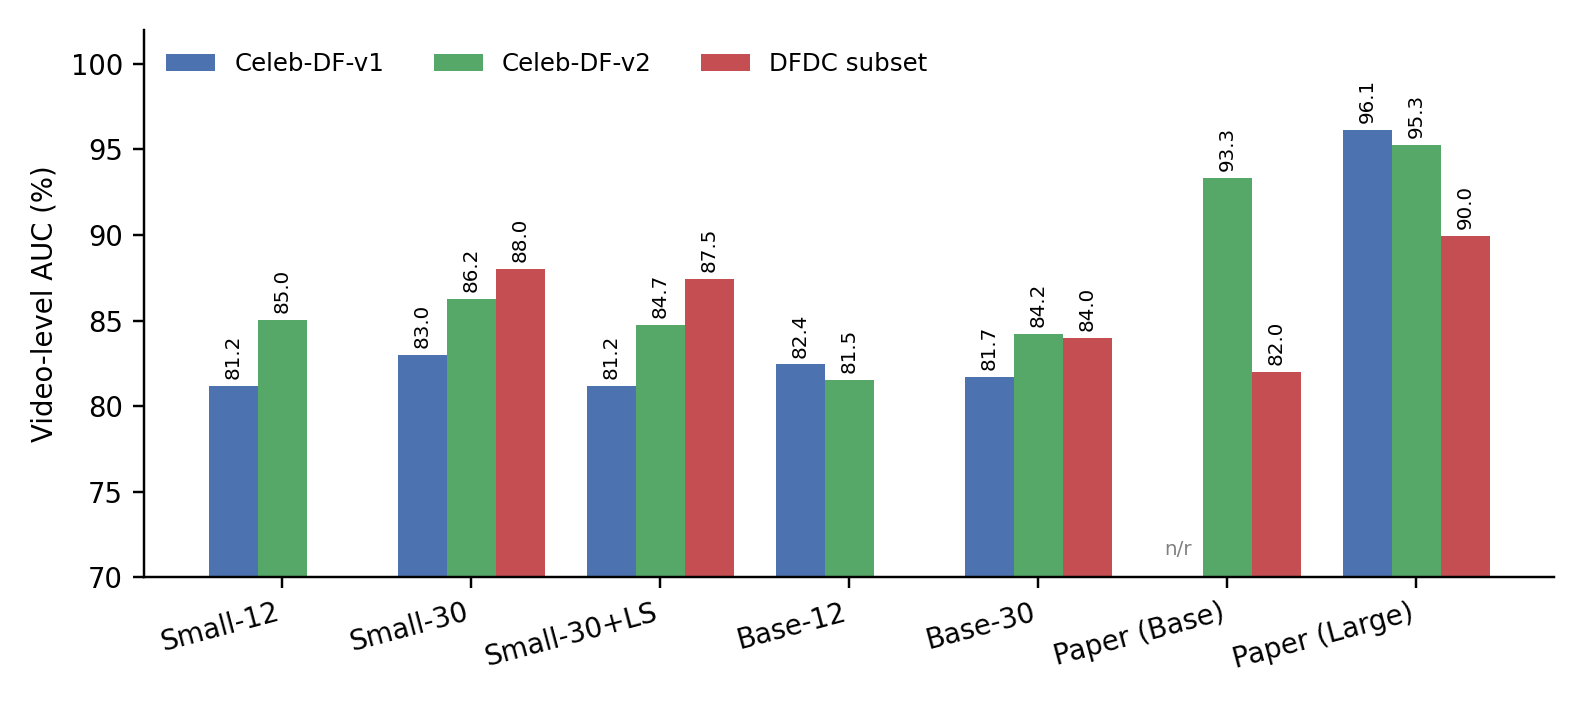
\includegraphics[width=0.78\textwidth]{fig_auc}
\caption{Cross-dataset video AUC of all configurations against the paper (n/r: not reported).}
\label{fig:auc}
\end{figure*}

\textbf{In-domain.} All our models reach 99.05--99.16\% FF++ validation AUC. This is within 0.4--0.5~pp of the paper's 99.56\% (test split), but the two numbers come from different splits. Our FF++ EER is about 3.2--3.6\% versus the paper's 1.79\%.

\textbf{Cross-dataset.} Our best model (Small, 30 epochs) is 13.16~pp below the paper on Celeb-DF-v1 and 9.01~pp below on Celeb-DF-v2, but only 1.93~pp below on our DFDC subset (Fig.~\ref{fig:gap}). Against the paper's own Base-size model, our Base is 9.13~pp lower on Celeb-DF-v2 and 2.00~pp higher on DFDC. The Celeb-DF generalization reported in the paper is therefore not reproduced in our setting, while the DFDC result is close. The DFDC comparison is weaker evidence: our subset (392 videos) may not be the paper's DFDC set.

\begin{figure}[!t]
\centering
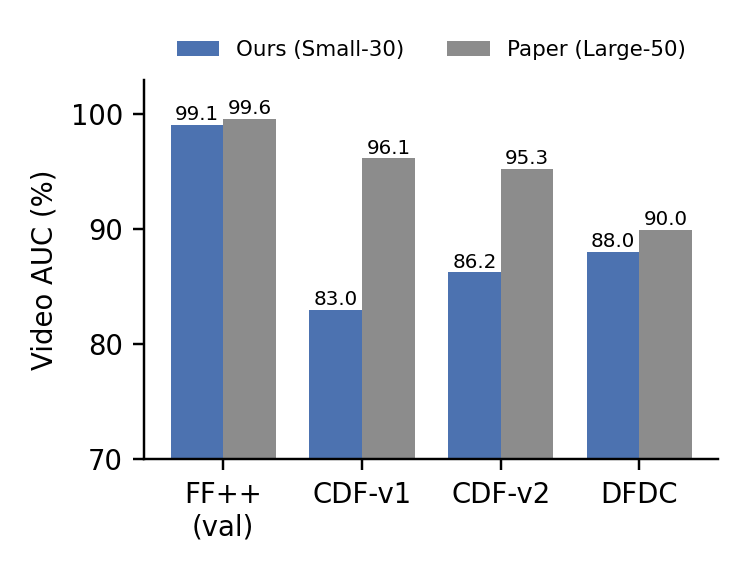
\includegraphics[width=2.9in]{fig_gap}
\caption{In-domain (FF++) versus unseen-dataset video AUC for Small, 30 epochs, and the paper (Large).}
\label{fig:gap}
\end{figure}

\subsection{Equal Error Rate}
\begin{table}[!t]
\caption{Cross-dataset EER (\%), lower is better.\label{tab:eer}}
\centering
\footnotesize
\setlength{\tabcolsep}{3pt}
\begin{tabular}{|l|c||c|c|c|}
\hline
Model & Ep. & CDF-v1 & CDF-v2 & DFDC\\
\hline
Small & 12 & 30.65 & 22.94 & --\\
\textbf{Small} & \textbf{30} & \textbf{26.32} & \textbf{22.35} & \textbf{19.74}\\
Small + LS & 30 & 26.32 & 25.00 & 19.94\\
Base & 12 & 25.81 & 26.18 & --\\
Base & 30 & 28.95 & 23.82 & 23.68\\
\hline
Paper (Base) & -- & n/r & 14.61 & 25.49\\
Paper (Large) & 50 & n/r & 12.65 & 17.96\\
\hline
\end{tabular}
\end{table}
Table~\ref{tab:eer} mirrors the AUC picture. Small at 30 epochs has the lowest EER among our models on Celeb-DF-v2 (22.35\% versus 12.65\% for the paper) and on DFDC (19.74\% versus 17.96\%). On Celeb-DF-v1 the 12-epoch Base model has a slightly lower EER (25.81\%) than Small-30 (26.32\%) although its AUC is lower (82.43\% versus 82.98\%); AUC and EER summarise different parts of the ROC curve and need not agree.

\subsection{DFDC subset}
\begin{table}[!t]
\caption{DFDC subset (392 videos, 12{,}544 frames), \texttt{best.pt} checkpoints.\label{tab:dfdc}}
\centering
\footnotesize
\begin{tabular}{|l||c|c|c|}
\hline
Metric & Small & Base & Better\\
\hline
Video AUC (\%) & \textbf{88.03} & 84.00 & Small\\
EER (\%) & \textbf{19.74} & 23.68 & Small\\
Frame AUC (\%) & \textbf{79.99} & 78.10 & Small\\
\hline
\end{tabular}
\end{table}
Small is ahead on all three metrics (Table~\ref{tab:dfdc}): $+4.03$~pp video AUC, $-3.94$~pp EER. Video-level AUC exceeds frame-level AUC by 8.04~pp (Small) and 5.90~pp (Base), consistent with averaging damping noisy single-frame predictions.

\textbf{Statistical uncertainty.} The subset is small and imbalanced (76 real, 316 fake). The Hanley--McNeil approximation~\cite{hanley1982meaning} gives a standard error of about 1.75~pp for an AUC of 88\%, i.e. a 95\% interval of roughly $\pm3.4$~pp. Small and Base are evaluated on the same videos, so their difference is paired and less uncertain than for independent samples, but the 4.03~pp gap and the 1.93~pp gap to the paper are both within or near this interval. Differences of 1--2~pp, which dominate the Celeb-DF comparisons (only 100 videos in v1), lie within sampling noise.

\section{Ablation Study}
All ablations change one factor relative to a stated reference; deltas are in pp.

\subsection{Training length (12 $\to$ 30 epochs)}
\begin{table}[!t]
\caption{Effect of 30 versus 12 epochs.\label{tab:epochs}}
\centering
\footnotesize
\setlength{\tabcolsep}{3pt}
\begin{tabular}{|l||c|c|c|c|}
\hline
Backbone & $\Delta$AUC v1 & $\Delta$EER v1 & $\Delta$AUC v2 & $\Delta$EER v2\\
\hline
Small & $+1.78$ & $-4.33$ & $+1.23$ & $-0.59$\\
Base & $-0.72$ & $+3.14$ & $+2.71$ & $-2.36$\\
\hline
\end{tabular}
\end{table}
Longer training helps Small on both Celeb-DF sets, but for Base the effect depends on the target dataset (Table~\ref{tab:epochs}). Training duration alone is not a reliable predictor of generalization. DFDC is not available for the 12-epoch models.

\subsection{Backbone size (Small versus Base)}
At 30 epochs, Base minus Small is $-1.27$~pp on Celeb-DF-v1, $-2.03$~pp on Celeb-DF-v2 and $-4.03$~pp on DFDC video AUC, even though Base has the higher FF++ validation AUC (99.16\% versus 99.08\%). At 12 epochs Base is $+1.23$~pp on v1 but $-3.51$~pp on v2. This differs from the paper's own Base-versus-Large comparison, where the larger model is better on Celeb-DF-v2 (+1.91~pp) and DFDC (+7.96~pp); the paper does not report a Small model.

\subsection{Label smoothing on the forgery-type loss}
\begin{table}[!t]
\caption{Small, 30 epochs: label smoothing 0.1 minus baseline.\label{tab:ls}}
\centering
\footnotesize
\begin{tabular}{|l||c|c|c|}
\hline
Dataset & $\Delta$ video AUC & $\Delta$ EER & $\Delta$ frame AUC\\
\hline
Celeb-DF-v1 & $-1.78$ & $0.00$ & n/a\\
Celeb-DF-v2 & $-1.51$ & $+2.65$ & n/a\\
DFDC subset & $-0.58$ & $+0.20$ & $+0.91$\\
\hline
\end{tabular}
\end{table}
The label-smoothed run (45{,}000 steps, best FF++ validation AUC 99.05\%) did not improve video AUC on any unseen set (Table~\ref{tab:ls}). DFDC frame-level AUC rose by 0.91~pp, so frame- and video-level results are not uniformly aligned. This is a single-seed result and does not show that label smoothing is generally ineffective. The baseline Celeb-DF numbers are final-checkpoint results whereas the label-smoothed evaluation used \texttt{best.pt}; this confound is disclosed in Section~\ref{sec:lim}.

\subsection{Auxiliary supervision and adapter design}\label{sec:paperabl}
The paper ablates the components that our code also supports (flags \texttt{--no\_aux}, \texttt{--variant lora} and \texttt{--variant linear}). Table~\ref{tab:paperabl} gives the paper's cross-dataset AUC for the same settings next to our full model.
\begin{table}[!t]
\caption{Paper's ablations~\cite{zhang2026dff} (Large backbone) and our corresponding full model; AUC (\%).\label{tab:paperabl}}
\centering
\footnotesize
\setlength{\tabcolsep}{3pt}
\begin{tabular}{|l||c|c|c|c|}
\hline
Setting (paper) & CDF-v1 & CDF-v2 & DFDC & Ours\\
\hline
Linear probe & 56.45 & 66.63 & 72.54 & \todo{run}\\
Plain LoRA & 85.14 & 85.14 & 79.95 & \todo{run}\\
No type loss ($\lambda_t{=}0$) & n/r & 90.93 & 84.44 & \todo{run}\\
Full DFF-Adapter & 96.14 & 95.26 & 89.96 & 82.98 / 86.25 / 88.03\\
\hline
\end{tabular}
\end{table}
In the paper, removing the type loss costs 4.33~pp on Celeb-DF-v2 and 5.52~pp on DFDC, and plain LoRA is 10.1~pp and 10.0~pp below the full model on those sets. \todo{insert our dff\_noaux, lora and linear results if they exist; they are not in the status report}

\section{Discussion}
\textbf{Source-domain accuracy is not robustness.} With about 99\% FF++ validation AUC, Small-30 loses 16.10~pp on Celeb-DF-v1, 12.8~pp on Celeb-DF-v2 and 11.05~pp on DFDC. A detector can separate real from fake very well on data like its training set and still struggle when the source, manipulation pipeline, compression or identity distribution changes. Which factor dominates cannot be determined from these experiments, and the FF++ and DFDC numbers may not belong to the same checkpoint.

\textbf{Where the gap to the paper is.} The shortfall is concentrated on Celeb-DF (9--13~pp), while on the DFDC subset we are within 2~pp of the paper's Large model. Candidate causes of the Celeb-DF gap are (i) backbone capacity (Small/Base versus Large), (ii) the training recipe (learning rate, weight decay, epochs), (iii) data and protocol differences (frames per video, splits, cropping, and the Celeb-DF lists), and (iv) implementation details. Several differ at once, so the comparison cannot attribute the gap to any one of them, and it does not by itself show that the paper is irreproducible or that our implementation is wrong. The parameter-count agreement with the paper's 3.5M budget and the unit tests against the literal equations support the adapter itself, but not the training recipe.

\textbf{Bigger is not automatically better.} In our runs Base wins on FF++ validation but loses to Small on DFDC on every metric. Plausible explanations (different learned representations, optimisation dynamics, interaction with the target data) remain hypotheses that need controlled runs. They also leave the paper's Base-versus-Large trend untested, since we have no Large run.

\textbf{Longer training and overfitting.} The mixed effect of 12 versus 30 epochs is consistent with overfitting to the source dataset, but it does not establish it.

\textbf{Label smoothing.} The data do not support a benefit at $\epsilon=0.1$ in this run. The paper itself notes that artifacts of different manipulation methods may overlap, which could make the auxiliary task noisy; smoothing was meant to soften that, but we did not measure type-classification quality, so we cannot say whether it did.

\section{Limitations}\label{sec:lim}
\begin{enumerate}
\item \textbf{Backbone mismatch.} The paper uses DINOv2-Large with registers; we use plain Small and Base, so the comparison does not isolate implementation quality.
\item \textbf{Training mismatch.} Epochs, learning rate, weight decay, frames per video and hardware differ from the paper, and the paper follows DeepFakeBench defaults.
\item \textbf{Evaluation protocol.} Our manifests (100, 518 and 392 videos) have not been verified to match the paper's benchmark splits. The DFDC subset is a subset, so its comparison with the paper's DFDC number is indicative only.
\item \textbf{Validation versus test.} Our FF++ column is validation AUC, whereas the paper reports AUC on the FF++ test split.
\item \textbf{Checkpoint inconsistency.} FF++ numbers are best-validation checkpoints, Celeb-DF numbers of baseline runs are final checkpoints, and DFDC and label-smoothing results use \texttt{best.pt}. The training durations behind each \texttt{best.pt} should be confirmed before treating Table~\ref{tab:auc} as a controlled comparison.
\item \textbf{Single seed.} No variance across seeds is available, so small differences cannot be separated from noise.
\item \textbf{No causal evidence.} The experiments show what changes, not why.
\item \textbf{Class imbalance and small $n$.} The DFDC subset has 76 real and 316 fake videos; Celeb-DF-v1 has only 100 videos. No confidence intervals beyond the approximation above were computed.
\item \textbf{Missing ablations.} Our own no-type-loss, plain-LoRA and linear-probe baselines are not reported (Section~\ref{sec:paperabl}).
\end{enumerate}

\section{Conclusion and Future Work}
We re-implemented DFF-Adapter on smaller DINOv2 backbones. In-domain FF++ AUC (99.08\% validation) is within about 0.5~pp of the paper's test AUC, but cross-dataset AUC on Celeb-DF is 9--13~pp lower, so the paper's Celeb-DF generalization is not reproduced in our setting. On a 392-video DFDC subset we are within 2~pp of the paper's Large model (88.03\% versus 89.96\%), with the caveat that the subsets may differ. Among our configurations Small trained for 30 epochs is the strongest cross-dataset candidate. A larger backbone and label smoothing on the type loss did not help. The most defensible conclusion is that source-dataset performance alone is insufficient to judge a deepfake detector.

\textbf{Future work.} (1) Evaluate one selected checkpoint per model on FF++ test and all unseen sets with a single scoring procedure. (2) Verify splits, cropping and the DFDC subset against DeepFakeBench. (3) Run at least three seeds for the best configuration. (4) Run the paper's ablations (no type loss, plain LoRA, linear probe) with our code and ablate label smoothing one factor at a time. (5) Evaluate the 12-epoch models on DFDC. (6) Try the paper's learning rate, weight decay and Large backbone if compute permits.

\bibliographystyle{IEEEtran}
\bibliography{ref}

{\appendix
\textbf{Platforms.} Training and evaluation ran as Kaggle notebooks on Tesla T4 GPUs (two GPUs used concurrently for two experiments); data were stored as private Kaggle datasets. Software: PyTorch, Hugging Face Transformers (\texttt{Dinov2Model}), OpenCV for image loading and augmentation, and MTCNN for face cropping. \todo{confirm library versions}

\textbf{Reliability measures.} The training script writes checkpoints atomically (temporary file, then rename) every 500 steps and at each epoch end, resumes mid-epoch from \texttt{last.pt} with a seed-and-epoch dependent sampler, stops cleanly after a maximum wall-clock time, and the runner evaluates a run only if \texttt{done.json} exists. These were used so that long runs under Kaggle's commit mode could be monitored and recovered.

\textbf{Prompts and AI assistance.} AI assistants (ChatGPT and Claude) were used to review and debug the training and runner code, to design the smoke test, and to draft this report from our experiment notes; all numbers were taken from our saved experiment results. \todo{confirm and list prompts if required}
}

\end{document}
